\chapter{Planificació}

En un primer moment, la planificació del projecte va ser la següent: \\

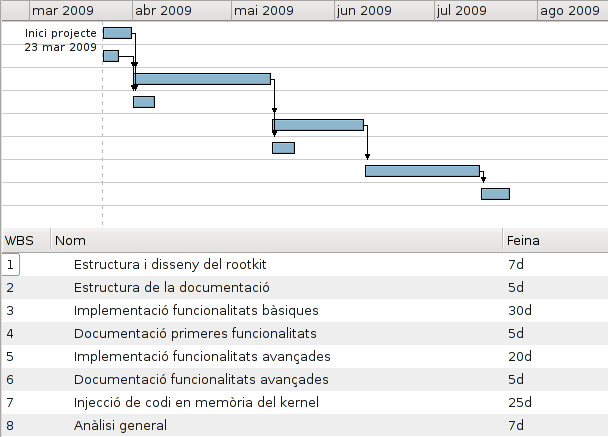
\includegraphics[scale=0.7,keepaspectratio]{primer_gantt.png} \\

Els punts principals d'aquesta planificació, eren el fet de no deixar la documentació del projecte pel final, 
sinó que fos un punt que s'anés avançant constantment. Varem separar les diferents tasques entre el disseny
i la recerca inicial, la implementació de les seves funcionalitats en dos blocs segons la seva dificultat,
una part del rootkit a nivell de kernel i només per a GNU/Linux, i finalment un anàlisis general per a polir-ho
i homogeneïtzar-ho tot. \\

Sabíem que el fet que gran part del projecte fos haver de fer la recerca, podia provocar alguns canvis en quant a
les funcionalitats decidides inicialment, i així va ser.

Sobre aquesta planificació, va haver-hi principalment els següents canvis:

\begin{itemize}
    \item Eliminació de la injecció de codi en memòria de kernel (Es va eliminar ja que en kernels actuals ja no 
        és factible, i per tant es va decidir potenciar altres punts. Tot i això s'ha documentat el què i el perquè)
    \item Falta de previsió en el fet que el planning passava per períodes d'examens finals i de vacances.
\end{itemize}

Com a comentaris importants, dir que la planificació inicial es va veure força afectada a partir de la tercera setmana de Juny, que al apropar-se
examens i entregues finals d'altres assignatures, varem pactar amb el tutor per a fer una petita pausa. També el període posterior
de vacances, va fer allargar-lo una mica més. \\

Un cop aplicats els diferents canvis que van afectar el projecte, la planificació final va ser la següent: \\

GRAFIC GANTT REAL
